% Options for packages loaded elsewhere
\PassOptionsToPackage{unicode}{hyperref}
\PassOptionsToPackage{hyphens}{url}
\PassOptionsToPackage{dvipsnames,svgnames,x11names}{xcolor}
%
\documentclass[
  letterpaper,
  DIV=11,
  numbers=noendperiod]{scrartcl}

\usepackage{amsmath,amssymb}
\usepackage{iftex}
\ifPDFTeX
  \usepackage[T1]{fontenc}
  \usepackage[utf8]{inputenc}
  \usepackage{textcomp} % provide euro and other symbols
\else % if luatex or xetex
  \usepackage{unicode-math}
  \defaultfontfeatures{Scale=MatchLowercase}
  \defaultfontfeatures[\rmfamily]{Ligatures=TeX,Scale=1}
\fi
\usepackage{lmodern}
\ifPDFTeX\else  
    % xetex/luatex font selection
\fi
% Use upquote if available, for straight quotes in verbatim environments
\IfFileExists{upquote.sty}{\usepackage{upquote}}{}
\IfFileExists{microtype.sty}{% use microtype if available
  \usepackage[]{microtype}
  \UseMicrotypeSet[protrusion]{basicmath} % disable protrusion for tt fonts
}{}
\makeatletter
\@ifundefined{KOMAClassName}{% if non-KOMA class
  \IfFileExists{parskip.sty}{%
    \usepackage{parskip}
  }{% else
    \setlength{\parindent}{0pt}
    \setlength{\parskip}{6pt plus 2pt minus 1pt}}
}{% if KOMA class
  \KOMAoptions{parskip=half}}
\makeatother
\usepackage{xcolor}
\setlength{\emergencystretch}{3em} % prevent overfull lines
\setcounter{secnumdepth}{-\maxdimen} % remove section numbering
% Make \paragraph and \subparagraph free-standing
\ifx\paragraph\undefined\else
  \let\oldparagraph\paragraph
  \renewcommand{\paragraph}[1]{\oldparagraph{#1}\mbox{}}
\fi
\ifx\subparagraph\undefined\else
  \let\oldsubparagraph\subparagraph
  \renewcommand{\subparagraph}[1]{\oldsubparagraph{#1}\mbox{}}
\fi


\providecommand{\tightlist}{%
  \setlength{\itemsep}{0pt}\setlength{\parskip}{0pt}}\usepackage{longtable,booktabs,array}
\usepackage{calc} % for calculating minipage widths
% Correct order of tables after \paragraph or \subparagraph
\usepackage{etoolbox}
\makeatletter
\patchcmd\longtable{\par}{\if@noskipsec\mbox{}\fi\par}{}{}
\makeatother
% Allow footnotes in longtable head/foot
\IfFileExists{footnotehyper.sty}{\usepackage{footnotehyper}}{\usepackage{footnote}}
\makesavenoteenv{longtable}
\usepackage{graphicx}
\makeatletter
\def\maxwidth{\ifdim\Gin@nat@width>\linewidth\linewidth\else\Gin@nat@width\fi}
\def\maxheight{\ifdim\Gin@nat@height>\textheight\textheight\else\Gin@nat@height\fi}
\makeatother
% Scale images if necessary, so that they will not overflow the page
% margins by default, and it is still possible to overwrite the defaults
% using explicit options in \includegraphics[width, height, ...]{}
\setkeys{Gin}{width=\maxwidth,height=\maxheight,keepaspectratio}
% Set default figure placement to htbp
\makeatletter
\def\fps@figure{htbp}
\makeatother
% definitions for citeproc citations
\NewDocumentCommand\citeproctext{}{}
\NewDocumentCommand\citeproc{mm}{%
  \begingroup\def\citeproctext{#2}\cite{#1}\endgroup}
\makeatletter
 % allow citations to break across lines
 \let\@cite@ofmt\@firstofone
 % avoid brackets around text for \cite:
 \def\@biblabel#1{}
 \def\@cite#1#2{{#1\if@tempswa , #2\fi}}
\makeatother
\newlength{\cslhangindent}
\setlength{\cslhangindent}{1.5em}
\newlength{\csllabelwidth}
\setlength{\csllabelwidth}{3em}
\newenvironment{CSLReferences}[2] % #1 hanging-indent, #2 entry-spacing
 {\begin{list}{}{%
  \setlength{\itemindent}{0pt}
  \setlength{\leftmargin}{0pt}
  \setlength{\parsep}{0pt}
  % turn on hanging indent if param 1 is 1
  \ifodd #1
   \setlength{\leftmargin}{\cslhangindent}
   \setlength{\itemindent}{-1\cslhangindent}
  \fi
  % set entry spacing
  \setlength{\itemsep}{#2\baselineskip}}}
 {\end{list}}
\usepackage{calc}
\newcommand{\CSLBlock}[1]{\hfill\break#1\hfill\break}
\newcommand{\CSLLeftMargin}[1]{\parbox[t]{\csllabelwidth}{\strut#1\strut}}
\newcommand{\CSLRightInline}[1]{\parbox[t]{\linewidth - \csllabelwidth}{\strut#1\strut}}
\newcommand{\CSLIndent}[1]{\hspace{\cslhangindent}#1}

\KOMAoption{captions}{tableheading}
\makeatletter
\@ifpackageloaded{caption}{}{\usepackage{caption}}
\AtBeginDocument{%
\ifdefined\contentsname
  \renewcommand*\contentsname{Table of contents}
\else
  \newcommand\contentsname{Table of contents}
\fi
\ifdefined\listfigurename
  \renewcommand*\listfigurename{List of Figures}
\else
  \newcommand\listfigurename{List of Figures}
\fi
\ifdefined\listtablename
  \renewcommand*\listtablename{List of Tables}
\else
  \newcommand\listtablename{List of Tables}
\fi
\ifdefined\figurename
  \renewcommand*\figurename{Figure}
\else
  \newcommand\figurename{Figure}
\fi
\ifdefined\tablename
  \renewcommand*\tablename{Table}
\else
  \newcommand\tablename{Table}
\fi
}
\@ifpackageloaded{float}{}{\usepackage{float}}
\floatstyle{ruled}
\@ifundefined{c@chapter}{\newfloat{codelisting}{h}{lop}}{\newfloat{codelisting}{h}{lop}[chapter]}
\floatname{codelisting}{Listing}
\newcommand*\listoflistings{\listof{codelisting}{List of Listings}}
\makeatother
\makeatletter
\makeatother
\makeatletter
\@ifpackageloaded{caption}{}{\usepackage{caption}}
\@ifpackageloaded{subcaption}{}{\usepackage{subcaption}}
\makeatother
\ifLuaTeX
  \usepackage{selnolig}  % disable illegal ligatures
\fi
\IfFileExists{bookmark.sty}{\usepackage{bookmark}}{\usepackage{hyperref}}
\IfFileExists{xurl.sty}{\usepackage{xurl}}{} % add URL line breaks if available
\urlstyle{same} % disable monospaced font for URLs
\hypersetup{
  pdftitle={How Do Household Energy Transitions Work?},
  pdfauthor={Jill Baumgartner (Co-PI); Sam Harper (Co-PI)},
  colorlinks=true,
  linkcolor={blue},
  filecolor={Maroon},
  citecolor={Blue},
  urlcolor={Blue},
  pdfcreator={LaTeX via pandoc}}

\title{How Do Household Energy Transitions Work?}
\author{Jill Baumgartner (Co-PI) \and Sam Harper (Co-PI)}
\date{2024-01-15}

\begin{document}
\maketitle
\renewcommand*\contentsname{Table of contents}
{
\hypersetup{linkcolor=}
\setcounter{tocdepth}{3}
\tableofcontents
}
\subsection{Abstract}\label{abstract}

\textbf{Introduction}

\textbf{Methods}

\textbf{Results}

\textbf{Conclusions}

Brief summary of what we did.

\subsection{Introduction}\label{introduction}

China is deploying an ambitious plan to transition up to 70\% of all
households in northern China to clean space heating, including Beijing.
To meet this target the Beijing municipal government announced a
two-pronged program that designates coal-restricted areas and
simultaneously offers subsidies to night-time electricity rates and for
the purchase and installation of electric-powered, air-source heat pumps
to replace traditional coal-heating stoves. The program is being rolled
out on a village-by-village basis; however there is uncertainty as to
when villages will receive the program. The variability in when the
policy is applied to each village allows us to treat the roll-out of the
program as a quasi-randomized intervention. Households may also be
differentially affected by this program due to factors such as financial
constraints, preferences and social capital, and there is uncertainty
about whether and how this intervention may affect indoor and outdoor
air pollution, as well as health behaviors and health outcomes.

\subsection{Background}\label{background}

\begin{itemize}
\tightlist
\item
  Context for the policy
\item
  Prior evidence on clean energy interventions
\item
  Importance of understanding mechanisms through which policies may
  affect outcomes.
\end{itemize}

\subsection{Specific Aims and Overarching
Approach}\label{specific-aims-and-overarching-approach}

This study used three data collection campaigns in winter 2018/19,
winter 2019/20, and winter 2021/22, as well as a partial campaign in
winter 2020/21 to advance the following aims:

\begin{enumerate}
\def\labelenumi{\arabic{enumi}.}
\item
  Estimate how much of the policy's overall effect on health, including
  respiratory symptoms and cardiovascular outcomes (blood pressure,
  central hemodynamics, blood inflammatory and oxidative stress
  markers), can be attributed to its impact on changes in PM2.5;
\item
  Quantify the impact of the policy on outdoor air quality and personal
  air pollution exposures, and specifically the source contribution from
  household coal burning (Previously Aim 3);
\item
  Quantify the contribution of changes in the chemical composition of
  PM2.5 from different sources to the overall effect on health outcomes
  (Previously Aim 2).
\end{enumerate}

\subsection{Study Design and Methods}\label{study-design-and-methods}

\begin{itemize}
\tightlist
\item
  Field equipment
\item
  DiD schematic
\item
  Mediation DAG
\end{itemize}

\subsubsection{Policy impacts}\label{policy-impacts}

To understand how Beijing's policy works we used a
difference-in-differences (DiD) design (Callaway 2020), leveraging the
staggered rollout of the policy across multiple villages to estimate its
impact on health outcomes and understand the mechanisms through which it
works. Simple comparisons of treated and untreated (i.e., control)
villages after the CBHP policy has been implemented are likely to be
biased by unmeasured village-level characteristics (e.g., migration,
average winter temperature) that are associated with health outcomes.
Similarly, comparisons of only treated villages before and after
exposure to the program are susceptible to bias by other factors
associated with changes in outcomes over time (i.e., secular trends,
impacts of the COVID-19 pandemic). By comparing \emph{changes} in
outcomes among treated villages to \emph{changes} in outcomes among
untreated villages, we can control for any unmeasured time-invariant
characteristics of villages as well as any general secular trends
affecting all villages that are unrelated to the policy

\begin{figure}

{\centering 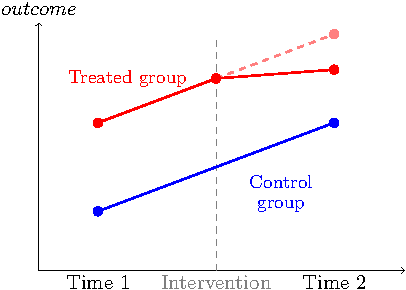
\includegraphics[width=0.7\textwidth,height=\textheight]{hei-report_files/figure-pdf/unnamed-chunk-1-1.pdf}

}

\caption{Stylized example of difference-in-differences}

\end{figure}%

The DiD design compares outcomes before and after an intervention in a
treated group relative to the same outcomes measured in a control group.
The control group trend provides the crucial ``counterfactual'' estimate
of what would have happened in the treated group had it not been
treated. By comparing each group to itself, this approach helps to
control for both measured and unmeasured fixed differences between the
treated and control groups. By measuring changes over time in outcomes
in the control group unaffected by the treatment, this approach also
controls for any unmeasured factors affecting outcome trends in both
treated and control groups. This is important since there are often many
potential factors affecting outcome trends that cannot be disentangled
from the policy if one only studies the treated group (as in a
traditional pre-post design).

The canonical DiD design (Card and Krueger 1994) compares two groups
(treated and control) at two different time periods (pre- and
post-intervention, Figure X). In the first time period both groups are
untreated, and in the second time period one group is exposed to the
intervention. If we assume that the differences between the groups would
have remained constant in the absence of the intervention (parallel
trends assumption), then an unbiased estimate of the impact of the
intervention in the post period can be calculated by subtracting the
pre-post difference in the untreated group from the pre-post difference
in the treated group.

However, when multiple groups are treated at different time periods, the
most common approach has been to use a two-way fixed effects model to
estimate the impact of the intervention which controls for secular
trends and differences between districts. However, recent evidence
suggests that the traditional two-way fixed effects estimation of the
treatment effect may be biased in the context of heterogeneous treatment
effects (Callaway and Sant'Anna 2021; Goodman-Bacon 2021)

\subsubsection{Pathways and mechanisms}\label{pathways-and-mechanisms}

To estimate how much of the CBHP intervention may work through different
mechanisms, we used causal mediation analysis. Causal approaches to
mediation attempt to discern between, and clarify the necessary
assumptions for identifying, different kinds of mediated effects. Taking
as an example the DAG in \textbf{Figure X}, with \(T\) as the policy,
\(M\) as PM\textsubscript{2.5}, and \(Y\) as systolic blood pressure, we
can define the controlled direct effect (\(CDE\)) as the effect of the
CBHP policy on systolic blood pressure if we fix the value of
PM\textsubscript{2.5} to a certain reference level for the entire
population. For example, we can estimate the impact of the policy on
health outcomes while holding PM\textsubscript{2.5} at a uniform level
of average background exposure, or some other hypothetical level.

\begin{figure}

{\centering 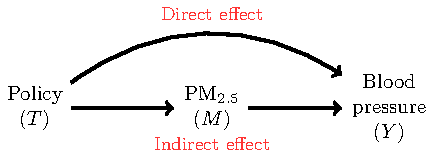
\includegraphics[width=0.7\textwidth,height=\textheight]{hei-report_files/figure-pdf/unnamed-chunk-2-1.pdf}

}

\caption{Example of direct and indirect effects with outcome (\(Y\)),
treatment (\(T\)), and mediator (\(M\))}

\end{figure}%

Although other mediated effects such as ``natural'' direct and indirect
effects are theoretically estimable (VanderWeele 2015), they involve
challenging ``cross-world'' assumptions that are difficult to anchor in
policy (Naimi et al. 2014). Other approaches to mechanisms have focused
on principal stratification (e.g., Zigler et al. 2016), although
conceptual difficulties with identifying the (unverifiable) principal
strata make it challenging for questions of mediation. Because
controlled direct effects are considered more directly policy relevant
for public health, we focus on estimating these mediated quantities.

\subsection{Data Analysis}\label{data-analysis}

\subsubsection{Total Effect}\label{total-effect}

To estimate the total effect of the policy we used a DiD analysis that
accommodates staggered treatment rollout. To allow for heterogeneity in
the context of staggered rollout we used `extended' two-way fixed
effects (ETWFE) models (Wooldridge 2021) to estimate the total effect of
the CBHP policy. The mean outcome (replaced by a suitable link function
\(g(\cdot)\) for binary or count outcomes) was defined using a set of
linear predictors:

\begin{equation}\phantomsection\label{eq-etwfe}{Y_{ijt}=g(\mu_{ijt}) = \alpha + \sum_{r=q}^{T} \beta_{r} d_{r} + \sum_{s=r}^{T} \gamma_{s} fs_{t}+ \sum_{r=q}^{T} \sum_{s=r}^{T} \tau_{rt} (d_{r} \times fs_{t}) + \varepsilon_{ijt}}\end{equation}

where \(Y_{ijt}\) is the outcome for individual \(i\) in village \(j\)
at time \(t\), \(d_{r}\) represent treatment cohort dummies, i.e., fixed
effects for cohorts of villages that were first exposed to the policy at
the same time \(q\) (e.g., in 2019, 2020, or 2021), \(fs_{t}\) are time
fixed effects corresponding to different winter data collection
campaigns (2018-19, 2019-20, or 2021-22), and \(\tau_{rt}\) are the
cohort-time \emph{ATTs}. The ETWFE and other approaches that allow for
several (potentially heterogenous) treatment effects may also be
averaged to provide a weighted \(ATT\). Several potential possibilities
are feasible, including weighting by treatment cohorts or time since
policy adoption (Goin and Riddell 2023)

\subsubsection{Mediation Analysis}\label{mediation-analysis}

As noted above, with respect to the mediation analysis we are chiefly
interested in the \(CDE\), which can be derived by adding relevant
mediators \(M\) to this model. If we also allow for exposure-mediator
interaction and potentially allow for adjustment for confounders \(W\)
of the mediator-outcome effect, we can extend equation
Equation~\ref{eq-etwfe} as follows:

\begin{equation}\phantomsection\label{eq-etwfem}{
\begin{aligned}
Y_{ijt}=g(\mu_{ijt}) = \alpha + \sum_{r=q}^{T} \beta_{r} d_{r} + \sum_{s=r}^{T} \gamma_{s} fs_{t}+ \sum_{r=q}^{T} \sum_{s=r}^{T} \tau_{rt} (d_{r} \times fs_{t}) \\ + \delta M_{it} + \sum_{r=q}^{T} \sum_{s=r}^{T} \eta_{rt} (d_{r} \times fs_{t} \times M_{it}) + \zeta \mathbf{W} + \varepsilon_{ijt}
\end{aligned}
}\end{equation}

where now \(\delta\) is the conditional effect of the mediator \(M\) at
the reference level of the treatment (again, represented via the series
of group-time interaction terms), and the collection of \(\eta\) terms
are coefficients for the product terms allowing for mediator-treatment
interaction. Finally, \(\zeta\) is a vector of coefficients for the set
of confounders contained within \(\mathbf{W}\).

As noted above, in the staggered DiD framework that allows for
heterogeneity we do not have a single treatment effect but a collection
of group-time treatment effects that may be averaged in different ways.
This extends to the estimation of the \(CDE\), in which case we will
also have several \(CDE\)s that can be averaged to make inferences about
the extent to which the policy's impact is mediated by
\emph{PM\textsubscript{2.5}}. Based on the setup in
Equation~\ref{eq-etwfem} the \(CDE\) is estimated as:
\(\delta + \eta_{rt}MT\). In the absence of interaction between the
exposure and the mediator (i.e., \(\eta_{rt}=0\)) the \(CDE\) will
simply be the estimated treatment effects
\(\sum_{r=q}^{T} \sum_{s=r}^{T} \tau_{rt}\), i.e., the effect of the
policy holding \(M\) constant. For a valid estimate of the \(CDE\) we
must account for confounding of the mediator-outcome effect, represented
by \(W\) in the equation above. Baseline measures of both the outcome
and the proposed mediators inherent in our DiD strategy will help to
reduce the potential for unmeasured confounding of the mediator-outcome
effect (Keele et al. 2015).

\subsection{Results}\label{results}

\subsubsection{Description of study sample
(Table)}\label{description-of-study-sample-table}

\begin{itemize}
\tightlist
\item
  Study flowchart of participants (Figure)
\item
  Description of PM measurements (Figure)
\item
  Uptake of the policy (Sankey energy use Figure)
\item
  Impact of `treatment assignment' on coal use (Figure? Table?)
\end{itemize}

\subsubsection{Aim 1: Policy impacts and potential
mediation}\label{aim-1-policy-impacts-and-potential-mediation}

\begin{itemize}
\tightlist
\item
  Impact of policy on PM mass (Figure)
\item
  Table of CDEs (Central SBP, Central DBP, FeNO, Respiratory outcomes,
  inflammatory markers), mediated by indoor PM (CDEs for personal and
  outdoor in SI)
\item
  Table for multiple mediation analysis for BP
\end{itemize}

\subsubsection{Aim 2: Source
contributions}\label{aim-2-source-contributions}

\begin{itemize}
\tightlist
\item
  Figure of source contributions (6 or fewer components)
\item
  Source contributions by treatment status
\item
  DiD for source contributions to PM
\end{itemize}

\subsubsection{Aim 3}\label{aim-3}

\begin{itemize}
\tightlist
\item
  Table of mediated health effects by source contribution (coal and
  biomass)
\end{itemize}

\subsection{Discussion and
Conclusions}\label{discussion-and-conclusions}

Other relevant results (Tables or figures in SI)

Policy impacts on other relevant outcomes:

\begin{itemize}
\tightlist
\item
  Temperature
\item
  Heating room
\item
  Well-being
\end{itemize}

\subsection{Implications of Findings}\label{implications-of-findings}

\subsection{Data Availability
Statement}\label{data-availability-statement}

To come\ldots{}

\subsection{Acknowledgements}\label{acknowledgements}

To come\ldots{}

\subsection{References}\label{references}

\subsection{Appendices}\label{appendices}

\subsection{About the authors}\label{about-the-authors}

\subsection*{Other publications}\label{other-publications}
\addcontentsline{toc}{subsection}{Other publications}

\phantomsection\label{refs}
\begin{CSLReferences}{1}{1}
\bibitem[\citeproctext]{ref-callaway2020}
Callaway B. 2020.
\href{https://doi.org/10.1007/978-3-319-57365-6_352-1}{Difference-in-{Differences}
for {Policy Evaluation}}. In: \emph{Handbook of {Labor}, {Human
Resources} and {Population Economics}} (K.F. Zimmermann, ed). {Springer
International Publishing}:{Cham}. 1--61.

\bibitem[\citeproctext]{ref-callaway2021}
Callaway B, Sant'Anna PHC. 2021. Difference-in-{Differences} with
multiple time periods. Journal of Econometrics 225:200--230;
doi:\href{https://doi.org/10.1016/j.jeconom.2020.12.001}{10.1016/j.jeconom.2020.12.001}.

\bibitem[\citeproctext]{ref-card1994}
Card D, Krueger AB. 1994. Minimum {Wages} and {Employment}: {A Case
Study} of the {Fast-Food Industry} in {New Jersey} and {Pennsylvania}.
American Economic Review 84: 772--93.

\bibitem[\citeproctext]{ref-goin2023}
Goin DE, Riddell CA. 2023. Comparing {Two-way Fixed Effects} and {New
Estimators} for {Difference-in-Differences}: {A Simulation Study} and
{Empirical Example}. Epidemiology 34:535;
doi:\href{https://doi.org/10.1097/EDE.0000000000001611}{10.1097/EDE.0000000000001611}.

\bibitem[\citeproctext]{ref-goodman-bacon2021}
Goodman-Bacon A. 2021. Difference-in-differences with variation in
treatment timing. Journal of Econometrics 225:254--277;
doi:\href{https://doi.org/10.1016/j.jeconom.2021.03.014}{10.1016/j.jeconom.2021.03.014}.

\bibitem[\citeproctext]{ref-keele2015}
Keele L, Tingley D, Yamamoto T. 2015. Identifying mechanisms behind
policy interventions via causal mediation analysis. Journal of Policy
Analysis and Management 34: 937--963.

\bibitem[\citeproctext]{ref-naimi2014}
Naimi AI, Kaufman JS, MacLehose RF. 2014. Mediation misgivings:
Ambiguous clinical and public health interpretations of natural direct
and indirect effects. International journal of epidemiology 43:1656--61;
doi:\href{https://doi.org/10.1093/ije/dyu107}{10.1093/ije/dyu107}.

\bibitem[\citeproctext]{ref-vanderweele2015}
VanderWeele TJ. 2015. \emph{Explanation in causal inference: Methods for
mediation and interaction}. {Oxford University Press}:{New York}.

\bibitem[\citeproctext]{ref-wooldridge2021}
Wooldridge JM. 2021. Two-{Way Fixed Effects}, the {Two-Way Mundlak
Regression}, and {Difference-in-Differences Estimators}.;
doi:\href{https://doi.org/10.2139/ssrn.3906345}{10.2139/ssrn.3906345}.

\bibitem[\citeproctext]{ref-zigler2016}
Zigler CM, Kim C, Choirat C, Hansen JB, Wang Y, Hund L, et al. 2016.
\emph{Causal inference methods for estimating long-term health effects
of air quality regulations. {Research} report 187.} {Health Effects
Institute / Health Effects Institute}:{Boston, MA}.

\end{CSLReferences}



\end{document}
